\part{Experimento}
O experimento desenvolvido neste trabalho consiste na criação de um jogo educacional utilizando a tecnologia HTML5. Como tecnologias complementares foram utilizadas: Javascript, CSS3, Queue.js, Highcharts e PhoneGap. O conteúdo educacional escolhido para ser trabalhado no jogo foi expressões algébricas. O jogo consiste em apresentar uma expressão ao jogador e pedir para que ele selecione e resolva cada uma das operações até chegar ao resultado final.

\chapter{Visão geral do fluxo}
O fluxo tem início quando o usuário acessa o jogo – como página de internet ou aplicativo para dispositivo móvel. O jogo inicializa e apresenta o botão “Play” para que o jogador comece os testes. Quando iniciados os testes o jogo escolhe uma expressão e a apresenta ao usuário para que ele selecione uma operação para resolver.

Assim que uma operação é selecionada o programa avalia se esta pode ser resolvida e apresenta a pontuação. Caso a operação selecionada não possa ser resolvida o programa se mantém no estado de seleção, no caso contrário o programa pede a solução para a operação selecionada. Depois que o usuário passa a solução o jogo apresenta a pontuação. Se a solução passada estiver incorreta o jogo permanece no estado de resolução, se a solução estiver correta a aplicação apresenta a expressão resultante.

Enquanto houver operações não resolvidas o fluxo se repete desde a seleção de operação. Quando não houver mais operações a serem resolvidas o programa apresenta os botões “Next...” e “Exit” para o jogador fazer o próximo teste ou sair do jogo respectivamente. Se o jogador for para o próximo teste o fluxo volta para o passo de escolha de expressão, no caso do jogador sair o programa apresenta a tela final.

\section{Inicialização da aplicação}
A função start é responsável pela inicialização da aplicação, recebe como parâmetro o identificador do elemento HTML que irá conter a tela do jogo e insere os principais elementos HTML do jogo, inclusive a tela inicial para que o usuário possa iniciar o jogo.

\section{Escolha da expressão}
A escolha da expressão é feita através da função newXp. Inicialmente a rotina seleciona uma expressão, escolhendo uma das disponibilizadas através do método startDB (executado no início dos testes) ou gerando uma com a função makeExp. Em seguida a expressão selecionada é passada para o contexto do jogo junto de suas soluções.

A criação de novas expressões leva em conta duas variáveis: número de operações e um conjunto de possíveis operações a serem utilizadas. As expressões são criadas de forma aleatória. A probabilidade para cada operação ser sorteada é 1 em n, onde n é o tamanho do conjunto de operações passado. 	Não existe restrição de unicidade para o conjunto de operações que são passadas para a função makeExp possibilitando alterar a probabilidade de que uma determinada operação seja escolhida.

Caso a expressão escolhida tenha sido gerada a fase de passar a expressão para o contexto do jogo envolve a avaliação da expressão para conhecer todas as soluções possíveis para a expressão. A avaliação da expressão é feita através de um algoritmo iterativo implementado na função evaluateTreeIt.

\section{Apresentação da expressão}
A expressão é apresentada utilizando a função appendXp que recebe como parâmetro a expressão e a imprime na tela utilizando a função htmlfy, uma função recursiva que retorna os elementos HTML que representam visualmente a expressão.

\section{Selecão da operação}
A seleção da operação é acionada através de um clique simples com o botão esquerdo do mouse ou toque (no caso de dispositivos móveis) sobre a operação. A função opClick é responsável por tratar tais eventos recebendo como parâmetro o identificador da operação. Internamente a função opClick faz uso da função select que é responsável por avaliar se a operação pode ou não ser resolvida.

\section{Pontuação}
Sempre que houver uma seleção ou tentativa resolver uma operação o jogo avalia se a ação está correta e então apresenta a pontuação através da função spanWarn que recebe como parâmetros o tipo de pontuação, perda ou ganho, e o respectivo valor.

Quando o jogador acerta uma seleção ou resolução na primeira tentavia ele recebe 1 ponto inteiro. Para cada erro o ponto é divido ao meio, assim que se o acerto ocorrer na segunda tentativa o jogador recebe meio ponto. A seleção da última operação não é pontuada por ser uma opção única.

\section{Pedido de solução}
Sempre que uma operação for selecionada corretamente o jogo pede ao usuário a solução através da função askForSolution que apresenta ao usuário a operação isolada seguida de uma caixa de texto, para que o usuário insira a solução daquela operação. Os elementos HTML apresentados contém aqueles retornados pela função htmlfy.

\section{Passagem da solução}
Depois que o usuário inserir a solução na caixa de texto e apertar a tecla ENTER ou tirar o foco da caixa de texto o programa faz uma avaliação da solução passada através da função solSubmit. Caso a solução esteja correta a caixa de texto é transformada em texto simples. Se houver mais de uma possível solução apenas aquela que foi resolvida permanece na tela, as outras são eliminadas da tela.

\section{Exemplo}
O exemplo a seguir exemplifica como o fluxo do jogo é percebido pelo usuário através da interface. Após inicializar a aplicação o usuário vê a tela inicial e o botão “Play”. Após apertar o botão “Play” o jogo apresenta uma expressão para o jogador resolver.

\begin{figure}[H]
	\caption{\label{xp_1} O sistema apresenta a expressão a ser resolvida}
	\begin{center}
	    
\includegraphics[scale=1]{xp_4_1.png}
	\end{center}
	\legend{Fonte: Produzido pelo autor}
\end{figure}

O jogador seleciona uma operação que não pode ser resolvida e perde metade da pontuação da seleção.

\begin{figure}[H]
	\caption{\label{miss_0_5_1}Jogador perde metade da pontuação da seleção}
	\begin{center}
	    
\includegraphics[scale=1]{miss_0_5.png}
	\end{center}
	\legend{Fonte: Produzido pelo autor}
\end{figure}

Em seguida o usuário seleciona a uma operação que pode ser resolvida e ganha a pontuação da seleção.

\begin{figure}[H]
	\caption{\label{score_0_5_1}Jogador ganha a pontuação da seleção}
	\begin{center}
	    
\includegraphics[scale=1]{score_0_5.png}
	\end{center}
	\legend{Fonte: Produzido pelo autor}
\end{figure}

O programa então apresenta a operação isolada e a caixa onde o usuário insere a solução. Este passo será omitido no resto do exemplo.

\begin{figure}[H]
	\caption{\label{xp_2}Programa pede a solução da operação}
	\begin{center}
	    
\includegraphics[scale=1]{xp_4_2_asksol_1.png}
	\end{center}
% 	\legend{Fonte: Produzido pelo autor}
\end{figure}

O jogador erra a solução e perde metade da pontuação da resolução.

\begin{figure}[H]
	\caption{\label{xp_3}O usuário insere um valor errado como solução}
	\begin{center}
	    
\includegraphics[scale=1]{xp_4_3_wrongans_1.png}
	\end{center}
	\legend{Fonte: Produzido pelo autor}
\end{figure}

\begin{figure}[H]
	\caption{\label{miss_0_5_2}O jogador perde metade dos pontos da solução}
	\begin{center}
	    
\includegraphics[scale=1]{miss_0_5.png}
	\end{center}
	\legend{Fonte: Produzido pelo autor}
\end{figure}

Em seguida o valor é corrigido e o usuário ganha a pontuação da solução.

\begin{figure}[H]
	\caption{\label{xp_4}O jogador insere a solução correta}
	\begin{center}
	    
\includegraphics[scale=1]{xp_4_4_rightans_1.png}
	\end{center}
	\legend{Fonte: Produzido pelo autor}
\end{figure}

\begin{figure}[H]
	\caption{\label{score_0_5_2}O sistema pontua o jogador pela solução}
	\begin{center}
	    
\includegraphics[scale=1]{score_0_5.png}
	\end{center}
	\legend{Fonte: Produzido pelo autor}
\end{figure}

O campo de texto é transformado em texto simples e a expressão resultante é apresentada ao usuário. O fluxo seleção/resolução se repete.

\begin{figure}[H]
	\caption{\label{xp_5}O sistema mostra a expressão resultante}
	\begin{center}
	    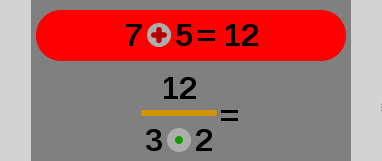
\includegraphics[scale=1]{xp_4_5.png}
	\end{center}
	\legend{Fonte: Produzido pelo autor}
\end{figure}

\begin{figure}[H]
	\caption{\label{score_1_1}O jogador recebe 1 ponto pelo acerto da seleção}
	\begin{center}
	    
\includegraphics[scale=1]{score_1.png}
	\end{center}
	\legend{Fonte: Produzido pelo autor}
\end{figure}

A divisão pode ser resolvida de duas maneiras e o jogo apresenta as duas possibilidades de solução.

\begin{figure}[H]
	\caption{\label{xp_7}O jogo aparesenta duas possibilidades de resolução para a divisão}
	\begin{center}
	    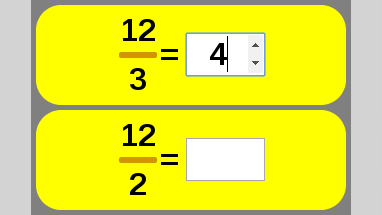
\includegraphics[scale=1]{xp_4_7_rightans_2.png}
	\end{center}
	\legend{Fonte: Produzido pelo autor}
\end{figure}

\begin{figure}[H]
	\caption{\label{score_1_2}O jogador recebe 1 ponto pelo acerto da solução}
	\begin{center}
	    
\includegraphics[scale=1]{score_1.png}
	\end{center}
	\legend{Fonte: Produzido pelo autor}
\end{figure}

O fluxo seleção/resolução se repete.

\begin{figure}[H]
	\caption{\label{xp_8}A nova expressão é apresentada ao usuário}
	\begin{center}
	    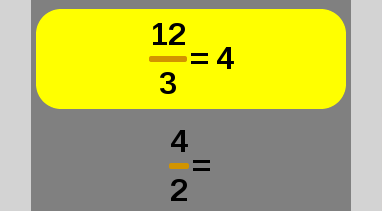
\includegraphics[scale=1]{xp_4_8.png}
	\end{center}
	\legend{Fonte: Produzido pelo autor}
\end{figure}

A seleção da última operação não é pontuada.

\begin{figure}[H]
	\caption{\label{score_0_1}A seleção da última operação não é pontuada}
	\begin{center}
	    
\includegraphics[scale=1]{score_0.png}
	\end{center}
	\legend{Fonte: Produzido pelo autor}
\end{figure}

\begin{figure}[H]
	\caption{\label{xp_10}O jogador insere a última solução a que está correta}
	\begin{center}
	    
\includegraphics[scale=1]{xp_4_10_rightans_3.png}
	\end{center}
	\legend{Fonte: Produzido pelo autor}
\end{figure}

\begin{figure}[H]
	\caption{\label{score_1_3}O jogador recebe a pontuação referente a solução}
	\begin{center}
	    
\includegraphics[scale=1]{score_1.png}
	\end{center}
	\legend{Fonte: Produzido pelo autor}
\end{figure}

	Não existem mais operações para serem resolvidas e as opções de continuar ou sair são apresentadas ao usuário.
	
\begin{figure}[H]
	\caption{\label{xp_11}A tela final é apresentada}
	\begin{center}
	    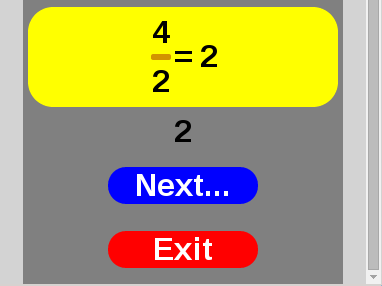
\includegraphics[scale=1]{xp_4_11.png}
	\end{center}
	\legend{Fonte: Produzido pelo autor}
\end{figure}

\chapter{Criação de expressões}

As expressões algébricas utilizadas são linguagens formais pois são um subconjunto de todas as palavras existentes para um determinado alfabeto. Para tanto existe pelo menos uma gramática capaz de gerar a linguagem formal envolvida.

	Toda gramática pode ser classificada de acordo com a Classificação de Chomsky onde toda gramática é pelo menos uma Gramática com Estrutura de Frase. A classe seguinte é um subconjunto da anterior e contém as Gramáticas Sensíveis ao Contexto. A classe das Gramáticas Livres de Contexto é novamente um subconjunto da classe anterior, assim como a ultima classe das Gramáticas Regulares é um subconjunto desta. A figura a seguir expressa a hierarquia existente entre as classes.
	
\begin{figure}[H]
	\caption{\label{gram_cls}Classes da Classificação de Chomsky e sua hierarquia}
	\begin{center}
	    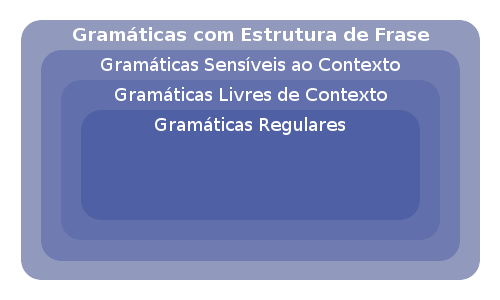
\includegraphics[scale=0.5]{driagrama_classes_gramaticas.png}
	\end{center}
	\legend{Fonte: Produzido pelo autor}
\end{figure}

A Classificação de Chomsky leva em conta os tipos de produções existentes na gramática. A seguir estão explicadas as classificações.

\section{Classificação de Chomsky}
Lembrando que as gramáticas são compostas por: um conjunto finito de símbolos não-terminais $N$, um conjunto finito de símbolos terminais $T$, um conjunto de produções $P$ e um símbolo inicial $\sigma$. A intersecção entre os conjuntos de símbolos não terminais e terminais deve ser vazia. O conjuto de produções é um subconjunto de todas as produções possíveis, o produto cartesiano de: todas as palavras geradas com símbolos não-terminais e terminais contendo pelo menos um símbolo não terminal (lado esquerdo da produção); todas as palavras geradas com símbolos não-terminais e terminais. O símbolo inicial deve pertencer ao conunto dos símbolos não terminais. Nas definições a seguir $\lambda$ denota a palavra nula.

\subsection{Gramáticas com Estrutura de Frase}
A gramática é com Estrutura de Frase se todas as produções são da forma:

$\alpha \to \delta$, onde $\alpha \in (N \cup T)$* - $T$*, $\delta \in (N \cup T)$*.

\subsection{Gramáticas Sensíveis ao Contexto}
A gramática é Sensível ao Contexto se todas as produções são da forma:

$\alpha A\beta \to \alpha \delta \beta$, onde $\alpha,\beta \in (N \cup T)$*$, A \in N, \delta \in (N \cup T)$* - \{$\lambda$\}.

\subsection{Gramáticas Livres de Contexto}
A gramática é Livre de Contexto se todas as produções são da forma:

$A \to \delta$, onde $A \in N, \delta \in (N \cup T)$*.

\subsection{Gramáticas Regulares}
A gramática é Regular se todas as produções são da forma:

$A \to a$ ou $A \to aB$ ou $A \to \lambda$.
